\section{使用 \OSname{} 多核的微基准测试}
\label{sec:benchmarks}


% We next evaluate the performance of \OSname{} on popular hardware. We published our benchmark code in~\cite{ariel-benchmarks}. 

% The \textbf{dual-core MCUs} we used are:
% \begin{enumerate*}[label=(\roman*)]
% \item Espressif \espsthree{} with dual Xtensa LX7 at 240 MHz, and 
% \item RP2040/RP2350 with dual Cortex-M0+/M33 at 133/150 MHz.
% \end{enumerate*}


% The \textbf{single-core boards} we used for comparison are:
% \begin{enumerate*}[label=(\roman*)]
% \item a Nordic nRF52840 with a Cortex-M4 at 64 MHz, and 
% \item an Espressif \espcthree{} with a RISC-V RV32IMC at 160 MHz.
% \end{enumerate*}
接下来,我们在主流的硬件平台上评估了 \OSname{} 的性能。我们的基准测试代码已发布在~\cite{ariel-benchmarks}。

我们使用的\textbf{双核 MCU}包括:
\begin{enumerate}[label=(\roman*)]
\item Espressif \espsthree{},配备双核 Xtensa LX7,主频 240 MHz;
\item RP2040/RP2350,配备双核 Cortex-M0+/M33,主频分别为 133 MHz 和 150 MHz。
\end{enumerate}

我们用于对比的\textbf{单核开发板}包括:
\begin{enumerate}[label=(\roman*)]
\item Nordic nRF52840,配备 Cortex-M4,主频 64 MHz;
\item Espressif \espcthree{},配备 RISC-V RV32IMC,主频 160 MHz。
\end{enumerate}
%\footnote{The benchmarks are available at \url{https://github.com/elenaf9/RIOT-rs-benchmarks}. The used commit revision is \textit{TODO}.} that compare the scheduler performance, quantify the speedup, and ...(\textit{TBC}).
\iffalse
We measured performance on the following popular boards, commercially available off-the-shelf: 
\begin{itemize}
    \item Nordic nRF52840: Arm Cortex\nobreakdash-M4, single-core, 64 MHz, 256 KB RAM, 1 MB Flash memory;
    \item Espressif \espcthree{}: RISC\nobreakdash-V RV32IMC, single-core, 160 MHz, 400 KB SRAM, 4 MB Flash memory;
    \item Espressif \espsthree{}: Xtensa LX7, dual-core, 240 MHz, 8 MB RAM, 16 MB Flash memory;
    \item RaspberryPi Pico: Arm Cortex\nobreakdash-M0+, dual-core,  133 MHz, 264 KB SRAM, 2 MB Flash memory.
\end{itemize}
\fi

% On Xtensa and Cortex-M, the performance is measured in ticks.
在 Xtensa 和 Cortex-M 架构上,性能是通过时钟周期(ticks)来衡量的。
\iffalse
\begin{itemize}
    \item Cortex-M: SysTick timer with the processor clock as the clock source
    \item Xtensa: CCOUNT cycle count registers
    % \item RISC-V: \noteEF{Unfortunately we can't measure the performance in ticks on the ESP32-C3 or ESP32-C6, because the \textit{mcycle} register isn't implemented on RV32IMC... Instead we have to use the system timer at 16Mhz... do we even need benchmark data for a second single-core board?}
\end{itemize}
\fi
% On the RISC-V-based \espcthree{}, we instead use the system timer, which runs at 16 MHz.
% The measurements we present are the average of 1000 runs.
在基于 RISC-V 的 \espcthree{} 上,我们使用系统定时器进行测量,该定时器运行频率为 16 MHz。
我们所展示的测量结果是 1000 次运行的平均值。
%, at 10\%  of the processor clock speed.
%Each benchmark consists of one or multiple threads, configured at the lowest priority, of which one executes the benchmark function.
% Results were deemed valid only if no timer/counter wrap-around and no thread migration of the benchmark-thread happened.% wrap, and the benchmarking thread didn’t migrate between cores. 



\subsection{比较多核调度器的差异}

%We compare the scheduler performance of the two global multicore scheduler implementations discussed in \ref{sec:design:scheduling} on dual-core platforms with each other, and against the baseline RIOT-rs scheduler. For this, a simple benchmark was implemented where two pairs of threads alternate in waking each other and then suspending their own execution by setting and waiting for thread flags. Hence, the benchmark largely consists of context switches.
% \autoref{fig:flags} depicts micro-benchmarks in which four threads, grouped into pairs, alternate in waking each other up and then suspending their own execution. % by setting and waiting for thread flags (hence the cost of context switches dominates here). 
% We compare the performance of different variants of the scheduler: (i) the \emph{single-core} variant described in \autoref{sec:single-core}, (ii) a multicore variant using \emph{core reallocation}, and (iii) a multicore variant using \emph{dynamic thread selection} as mentioned in \autoref{sec:Assigning-Threads-to-Cores}. 

\autoref{fig:flags} 展示了一个微基准测试,其中四条线程被分为两组,交替唤醒对方并挂起自己的执行。% 通过设置和等待线程标志(因此上下文切换的成本在这里占主导地位)。
我们比较了不同调度器变体的性能:(i) 在 \autoref{sec:single-core} 中描述的 \emph{单核} 变体,(ii) 使用 \emph{核重分配} 的多核变体,以及 (iii) 在 \autoref{sec:Assigning-Threads-to-Cores} 中提到的使用 \emph{动态线程选择} 的多核变体。


\pgfplotstableread[col sep=comma,]{translate/data/flags_dual-core_espressif-esp32-s3-devkitc-1.csv}\flagsdualesp{}
\pgfplotstableread[col sep=comma,]{translate/data/flags_dual-core_rpi-pico.csv}\flagsdualpico{}
\pgfplotstableread[col sep=comma,]{translate/data/flags_dual-core_rpi-pico2.csv}\flagsdualpicotwo{}
\begin{figure}[t!]
     \begin{subfigure}[t]{0.49\columnwidth}
     \begin{tikzpicture}
         {
            \begin{axis}[
            ybar,
            ourybarstyle,
            bar width=8pt,
            enlarge x limits=0.2,
            height=4cm, width=\textwidth,
            ylabel={Ticks},
            ytick distance=1000,
            symbolic x coords={{Single Core},{Multicore (Reallocation)},{Multicore (Dynamic)}},
            xticklabels={{Single Core},{Multicore\\(Reallocation)},{Multicore\\(Dynamic)}},
            nodes near coords style={font=\small, black, rotate=70, anchor=south east, yshift=-6pt, xshift=+27pt},
            xticklabel style={font=\small, rotate=45, anchor=east, align=right},
        ]
      \addplot table [y index=1]{\flagsdualpico};
      \addplot table [y index=1]{\flagsdualpicotwo};
    \end{axis}}
    \end{tikzpicture}
    \caption{RP2040/RP2350 (blue/purple)\label{fig:flags_rp2040}}
     \end{subfigure}
     \begin{subfigure}[t]{0.49\columnwidth}
     \begin{tikzpicture}
         {
            \begin{axis}[
            ybar,
            ourybarstyle,
            bar width=15pt,
            enlarge x limits=0.2,
            height=4cm, width=\textwidth,
            ylabel={Ticks},
            ytick distance=1000,
            symbolic x coords= {{Single Core},{Multicore (Reallocation)},{Multicore (Dynamic)}},
            xticklabels={{Single Core},{Multicore\\(Reallocation)},{Multicore\\(Dynamic)}},
            nodes near coords style={font=\small, black, rotate=45, anchor=south west, xshift=-2pt},
            xticklabel style={font=\small, rotate=45, anchor=east, align=right},
        ]
      \addplot table [y index=1]{\flagsdualesp};
    \end{axis}}
    \end{tikzpicture}
    \caption{ESP32-S3 (dual Xtensa LX7)\label{fig:flags_esp32s3}}
    \end{subfigure}
    \caption{两种多核调度器设计的上下文切换性能与单核配置的对比 \label{fig:flags}}
\end{figure}

% The results show that \textit{dynamic} outperforms \textit{reallocation} on all the multicore microcontrollers we tested.

% The results show that \textit{dynamic} outperforms \textit{reallocation} on both microcontrollers we tested. 
% The relatively more complex \textit{reallocation} routine, executed after each thread state change, takes a toll. 
% We notice a degradation of the performance of \textit{reallocation} versus single-core on RP2040, whereas speedups are observed on \espsthree{}. %This can be explained by different degrees of parallelization on the two platforms.

结果表明,在我们测试的所有多核微控制器上,动态分配优于重新分配。相对复杂的重新分配例程在每次线程状态变化后执行,会带来一定的代价。

\iffalse
\begin{enumerate}
    \item The \textit{Dynamic} approach outperforms the \textit{Reallocation} on both platforms.
    \item On the RP2040, no significant speedup was achieved through the multicore configuration, and even a degradation in case of the \textit{Dynamic} approach. On the \espsthree{}, the speedup is a factor of 1.3 in the \textit{Reallocation} approach and 1.5 for the \textit{Dynamic} one.
\end{enumerate}
\fi
%(1) is likely due to the complexity of the \textit{reallocation} routine, which is executed after each thread state change. The findings in (2) can be explained by different degrees of parallelization on the two platforms.
%As discussed in \autoref{sec:design:sync}, \OSname{} applies mutual exclusion to the whole kernel, and thus %no parallelization in the scheduler is possible.
% The benchmark largely consists of scheduler operations. Thus, mutual exclusion in the scheduler forces mostly sequential execution on the RP2040.
% In contrast, on the \espsthree{}, parallelization happens differently in hardware, forcing sequential execution less often. %however, 
% Furthermore, one benchmark iteration on \espsthree{} requires
% many more ticks than on the RP2040.
% Thus, \espsthree{} reaps more benefits from parallelization in this benchmark.
% %If we assume that this can be at least partly 
% %linked to a larger cost of the scheduler interrupt (and the saving and restoring of the trap frame). Thus, this larger segment that can run independently between the cores on this platform reaps more benefits from parallelization.
% In the following, we focus on the \textit{dynamic thread selection} variant for our multicore scheduling.
该基准测试主要由调度器操作构成。因此,RP2040上的调度器互斥机制导致其主要以顺序方式执行。
相比之下,在\espsthree{}上,硬件层面的并行化机制有所不同,较少强制执行顺序操作。此外,\espsthree{}上完成一次基准测试迭代所需的时钟周期远多于RP2040。因此,在此基准测试中,\espsthree{}能够从并行化中获得更多优势。
接下来,我们将重点关注多核调度中的\textit{动态线程选择}结构。
%approach, which we study further in the following.
% for our final SMP implementation. We furthermore found this approach to be the simpler and more intuitive one of the two, although additional care must be taken due to the lack of a global state. The following subsections use the \textit{dynamic} scheduler implementations for multicore.

% \iffalse
% \begin{figure}[htbp]
%      \begin{subfigure}[t]{0.49\columnwidth}
%     \centering
%          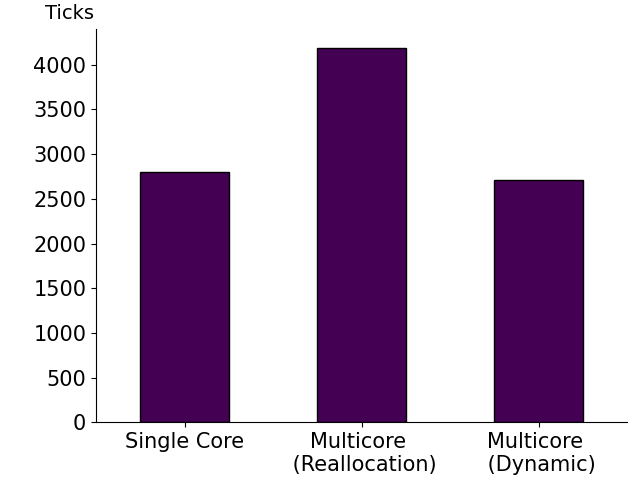
\includegraphics[width=\textwidth]{figures/flags_dual-core_rpi-pico.png}
%          \caption{RP2040 (dual Cortex-M0+)\label{fig:flags_rp2040}}
%      \end{subfigure}
%      \hfill
%      \begin{subfigure}[t]{0.49\columnwidth}
%          \centering
%          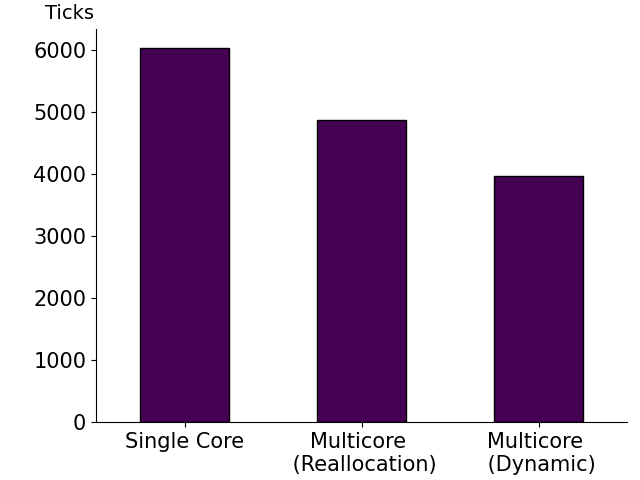
\includegraphics[width=\textwidth]{figures/flags_dual-core_espressif-esp32-s3-wroom-1.png}
%          \caption{ESP32-S3 (dual Xtensa LX7)\label{fig:flags_esp32s3}}
%      \end{subfigure}
%     \caption{Context switching performance of the two multicore scheduler designs compared with single-core configuration~.\label{fig:flags}}
% \end{figure}
% \fi
\subsection{多核调度的开销}

% We next measure
% the overhead of our multicore scheduling feature, compared to the single-core scheduler we started from in \autoref{sec:single-core}.
% For this, we focus on thread preemption, because, compared to single-core, the multicore feature adds an additional step: inserting the preempted thread back into the runqueue. %, whereas in the case of single-core this step is skipped.
% \autoref{fig:preempt} reports on micro-benchmarks performed on different single-core boards, in which a lower-priority thread sets the flag for a higher-priority thread, resulting in a context switch.

% We observe that the overhead when the multicore feature is enabled remains quite small, approx. 9.6\% on the nRF52840 and 5.3\% on the \espcthree{}. 
% Conveniently, we can therefore enable multicore by default

% in \OSname{}.

接下来,我们测量多核调度功能的开销,并将其与我们在\autoref{sec:single-core}中开始时的单核调度器进行比较。为此,我们专注于线程抢占,因为与单核相比,多核功能增加了一个额外的步骤:将被抢占的线程重新插入运行队列。%而在单核情况下,此步骤会被跳过。
\autoref{fig:preempt}报告了在不同单核开发板上进行的微基准测试结果,其中低优先级线程设置了一个标志以触发高优先级线程的运行,从而导致上下文切换。
我们观察到,启用多核功能时的开销仍然很小,在nRF52840上约为9.6%,在\espcthree{}上约为5.3%。因此,我们可以在\OSname{}中默认启用多核功能。

\pgfplotstableread[col sep=comma,]{translate/data/preempt_both_ai-c3.csv}\preemptesp{}
\pgfplotstableread[col sep=comma,]{translate/data/preempt_both_nrf52840dk.csv}\preemptnrf{}
\begin{figure}[t!]
     \begin{subfigure}[t]{0.49\columnwidth}
     \begin{tikzpicture}
         {
            \begin{axis}[
            ybar,
            ourybarstyle,
            bar width=20pt,
            enlarge x limits=0.4,
            height=4cm, width=\textwidth,
            ylabel={Ticks},
            ytick distance=200,
            symbolic x coords={{Multicore scheduler disabled},{Multicore scheduler enabled}},
            xticklabels={{disabled},{enabled}},
            nodes near coords style={font=\small, black, rotate=45, anchor=south west, xshift=-2pt},
            xticklabel style={font=\small, align=center},
        ]
      \addplot table [y index=1]{\preemptnrf};
    \end{axis}}
    \end{tikzpicture}
         \caption{nRF52840 (Cortex-M4)\label{fig:preempt_nrf52840}}
     \end{subfigure}
     \begin{subfigure}[t]{0.49\columnwidth}
     \begin{tikzpicture}
         {
            \begin{axis}[
            ybar,
            ourybarstyle,
            bar width=20pt,
            enlarge x limits=0.4,
            height=4cm, width=\textwidth,
            ylabel={Ticks},
            ytick distance=50,
            symbolic x coords={{Multicore scheduler disabled},{Multicore scheduler enabled}},
            xticklabels={{disabled},{enabled}},
            nodes near coords style={font=\small, black, rotate=45, anchor=south west, xshift=-2pt},
            xticklabel style={font=\small, align=center},
        ]
      \addplot table [y index=1]{\preemptesp};
    \end{axis}}
    \end{tikzpicture}
         \caption{ESP32-C3 (RISC-V)\label{fig:preempt_esp32c3}}
    \end{subfigure}
    \caption{在单核硬件上测量的多核调度特性开销 %when a running thread is being preempted on a single-core board.
    \label{fig:preempt}}
\end{figure}
% \iffalse
% \begin{figure}[htbp]
%      \begin{subfigure}[t]{0.24\textwidth}
%          \centering
%          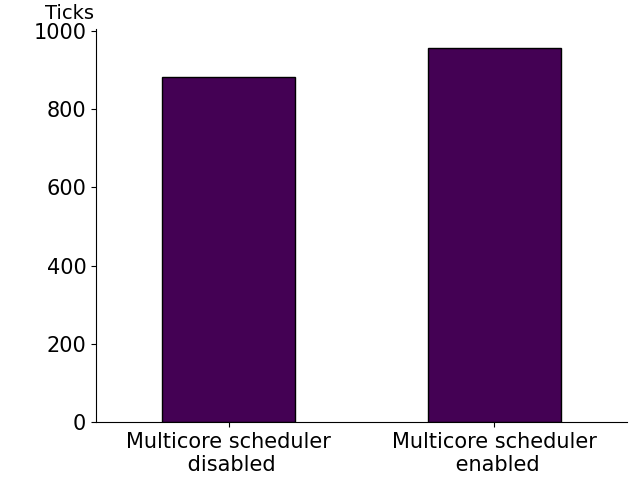
\includegraphics[width=\textwidth]{figures/preempt_both_nrf52840dk.png}
%          \caption{nRF52840 (Cortex-M4)\label{fig:preempt_nrf52840}}
%      \end{subfigure}
%      \hfill
%      \begin{subfigure}[t]{0.24\textwidth}
%          \centering
%          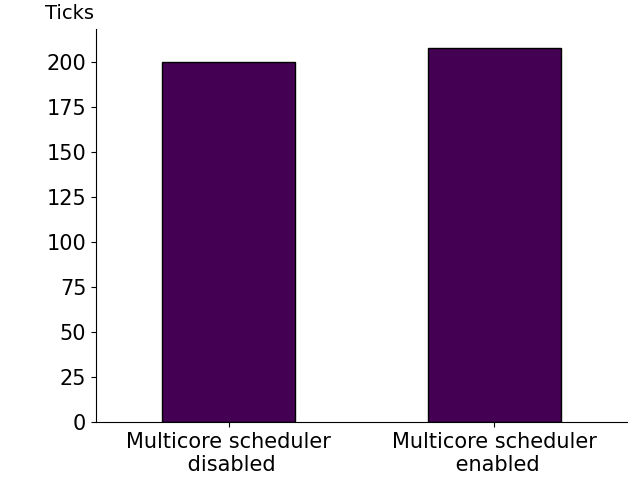
\includegraphics[width=\textwidth]{figures/preempt_both_ai-c3.png}
%          \caption{ESP32-C3 (RISC-V)\label{fig:preempt_esp32c3}}
%      \end{subfigure}
%     \caption{Overhead of the multicore scheduling feature when a running thread is being preempted.\label{fig:preempt}}
% \end{figure}
% \fi  

\subsection{计算密集型任务的加速}

\pgfplotstableread[col sep=comma,]{translate/data/matrix-mult_speedup_espressif-esp32-s3-devkitc-1.csv}\matrixesp{}
\pgfplotstableread[col sep=comma,]{translate/data/matrix-mult_speedup_rpi-pico.csv}\matrixpico{}
\pgfplotstableread[col sep=comma,]{translate/data/matrix-mult_speedup_rpi-pico2.csv}\matrixpicotwo{}
\begin{figure}[t]  
     \begin{subfigure}{0.49\columnwidth}
     \begin{tikzpicture}                                                   
         {
            \begin{axis}[                  
            ourlinestyle,              
            height=4cm, width=\textwidth,  
            ylabel={Relative speedup},     
            ytick distance=0.5,         
            tension=0.1,                
        ]                               
        \addplot+[myTeal, mark options={fill=myTeal}] table [x=0, y=speedup] {\matrixpico};                    
        \addplot+[myEggplant, mark options={fill=myEggplant}] table [x=0, y=speedup] {\matrixpicotwo};
    \end{axis}}                           
    \end{tikzpicture}      
     \caption{RP2040/RP2350 (blue/purple)\label{fig:matrix-mult_rp2040}}
     \end{subfigure}                                                   
     \begin{subfigure}{0.49\columnwidth}                                                                            
     \begin{tikzpicture}                                                                                                          
         {                                                                                                              
            \begin{axis}[                                                                                    
            ourlinestyle,                                                                             
            height=4cm, width=\textwidth,
            ylabel={Relative speedup},
            ytick distance=0.5,
        ]
        \addplot+[myTeal, mark options={fill=myTeal}] table [x=0, y=speedup] {\matrixesp};
    \end{axis}}             
    \end{tikzpicture}
         \caption{ESP32-S3 (dual Xtensa LX7)\label{fig:matrix-mult_esp32s3}}
    \end{subfigure}                                                             
    \caption{\(N\times N\) 矩阵的乘积, \(N\in\{10, 20, ...,  80\}\)\label{fig:matrix-mult}}
\end{figure}  
% We next benchmark 
% $N\times N$ matrix multiplication, with and without the multicore feature. 
% In the single-core configuration, the two computations are executed sequentially.
% For multicore, the tasks are distributed to two threads that are scheduled in parallel.
% We observe in Fig.~\ref{fig:matrix-mult} that when $N$ is small, IPC overhead dominates parallelization gains. When $N$ grows larger, we observe a performance gain tending towards 2x.
% We also notice that performance gains are not strictly linear. This is subject for further investigation --- it might be due to MCU-specific memory subsystem characteristics. %, subject to further investigation. 
% For example, on the RP2040, both cores compete for a shared memory bus~\cite{pico-mem-layout}.
接下来,我们分别在启用和未启用多核功能的情况下, 进行了 $N\times N$ 矩阵乘法的基准测试。在单核配置中,两次计算是顺序执行的。对于多核配置,任务被分配到两个线程中,并且这两个线程是并行调度的。
从图~\ref{fig:matrix-mult}中我们可以观察到,当 N 较小时,IPC(进程间通信)开销主导了并行化的收益。而当 N 增大时,我们观察到性能提升逐渐趋于 2 倍。我们还注意到性能提升并非严格线性增长。这有待进一步研究——它可能是由于 MCU(微控制器)特定的存储子系统特性所导致的。例如,在 RP2040 上,两个核会竞争共享的内存总线~\cite{pico-mem-layout}。
% \noteEF{For the record: It could still be that the speedup tends towards 2x if we test larger matrix sizes, e.g. 50x50. However, we can't do that with our benchmark because the timer wraps before the computation is completed.}

\textbf{总结 ---} 通过采用全局调度方案和优先级机制,我们实现了\emph{持续工作}和\emph{实时性}特性。我们的硬件抽象提供了\emph{可移植性},并且我们通过实验测量展示了\emph{透明性}。因此,我们已经实现了我们在第~\ref{sec:goals}节中设定的目标。
% \iffalse
% \begin{figure}[b!]
%      \centering
%      \begin{subfigure}[t]{0.24\textwidth}
%          \centering
%          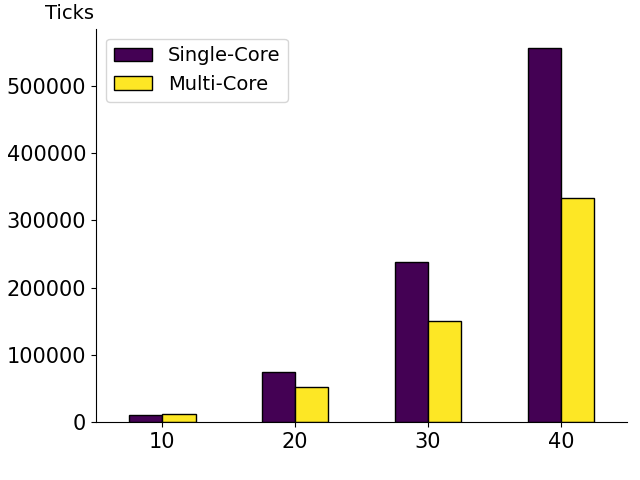
\includegraphics[width=\textwidth]{figures/matrix-mult_dual-core_rpi-pico.png}
%          \caption{RP2040\label{fig:matrix-mult_rp2040}}
%      \end{subfigure}
%      \hfill
%      \begin{subfigure}[t]{0.24\textwidth}
%          \centering
%          \includegraphics[width=\textwidth]{figures/matrix-mult_dual-core_espressif-esp32-s3-devkitc-1.png}
%          \caption{ESP32-S3\label{fig:matrix-mult_esp32s3}}
%      \end{subfigure}
%     \caption{Matrix-Multiplication performance of single- vs multicore for NxN matrices, \(N\in\{10, 20, 30, 40\}\)\label{fig:matrix-mult}}
% \end{figure}
% \fi
                             



%\textbf{Summary ---} Multicore scheduling overhead compared to a single-core scheduling variant is measurable but minor, thus the multicore variant can be the default on all platforms. In practice, parallel computation speedup with multicore scheduling is indeed substantial: we measured up to 175\% on dual core. \emph{Dynamic thread selection} outperforms other multicore variants, so we chose it as our default in \OSname{}. 
 %\noteEB{Kaspar TO DO: check the summary}